\documentclass[11pt]{article}

\usepackage{fullpage}
\usepackage[utf8]{inputenc}
\usepackage{graphicx}

\title{ARM Final Report}
\author{Diego Cupello      (dc1020)\\
Norberto Mateos Camara     (nm920)\\
Andrey Popov               (ap4220)\\
Agustin Sotero Bourel      (as1920)\\}

\begin{document}

\maketitle
\thispagestyle{empty}
\newpage
\setcounter{page}{1}
\section{Assembler Implementation}

We decided to implement the assembler using two-pass assembly, which we thought we could implement more efficiently as the JMC students could work on the first pass and getting the instructions ready to process for the second pass, while the computing students could be working on translating the instructions as they had a better understanding of assembly. The first pass creates a symbol table by reading through the lines of an assembly file and adding a new label with its corresponding address to the symbol table when the current line is a label, during this first pass we also count the number of instructions (which excludes the labels), the number of instructions is then used to initialise the array of instructions to be filled with the second pass. \\

The symbol table created is represented with a dedicated data structure symtable.h with its implementation in symtableimpl.c (both files are located in the data structures folder of src). Our symbol table is implemented as a linked list, that contains pointers to the first and last nodes, each node contains a label and its corresponding address. Inside symtableimpl.c are defined functions needed to access, print, allocate and free the contents of a symbol table. \\

The second pass fills an instruction array of unsigned 32-bit integers with the binary instructions, as well as a queue of ldr data (represented by a first in first out queue data structure). To do this it reads again the input assembly file and calls the assembleInstruction function in inassembler.c if the current line is an instruction. assembleInstruction then checks what type of instruction the current one is and calls the corresponding function (also located in inassembler.c). Each assembly function then returns the corresponding 32-bit instruction which is added to the instruction array. An exception is if the instruction is a LDR transfer instruction with a numeric constant of the form $<$=expression$>$ which adds the expression to the queue. This is in order to be able to handle storing various values in the data at the end of the binary file. \\

Finally the function writeBinFile is called which writes all the instruction in the instruction array directly to the binary file, it then writes the contents of the fifo queue at the end of the file. The resulting binOut file is the assembled binary file. \\

\begin{figure}[htp]
    \centering
    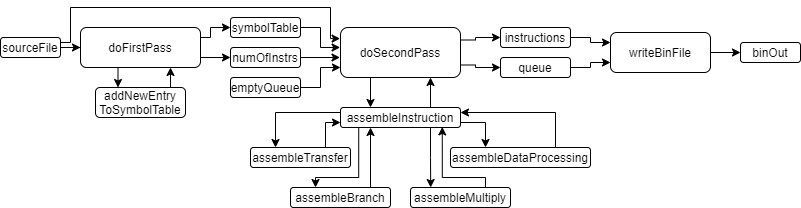
\includegraphics[width=17cm]{Assembler.png}
    \caption{Assembler Data Flow Diagram}

\end{figure}
\newpage

\begin{figure}[htp]
    \centering
    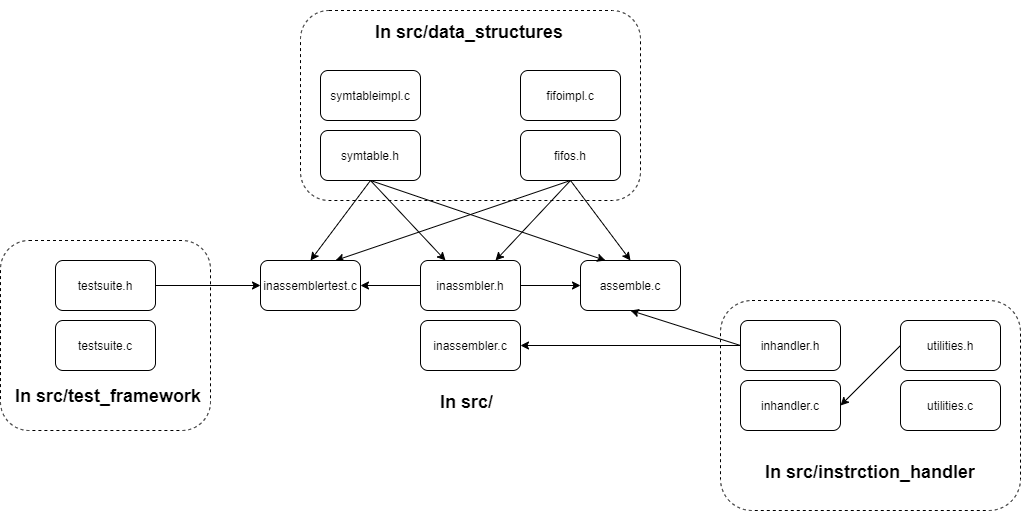
\includegraphics[width=17cm]{assemblerd.png}
    \caption{Assembler Dependencies Diagram}
\end{figure}


\section{Extension Overview}
Our extension consists of two parts, a debugger for assembly files and support for block data transfer instructions in both the assembler and the emulator. The debugger is inspired by the GNU debugger for C, but it is implemented to debug assembly files being able to monitor registers and memory of our emulated ARM machine. An assembly file is debugged by running it (r) (This runs the program, and then works like the command continue (c) in GDB) or executing the next line (n), a user can also set breakpoints (b \{Line\#\}) and watchpoints (w R\{register\#\}), remove breakpoints (rb \{Line\#\}) and watchpoints (rw R\{register\#\}). The debugger can also print the contents of a specific register (p R\{register\#\}) or address (p \{address\}), or similarly to the output of the emulator in part 1 (p all) prints the current state of the ARM machine, finally a user can exit the debugger using (q).\\

\begin{figure}[htp]
    \centering
    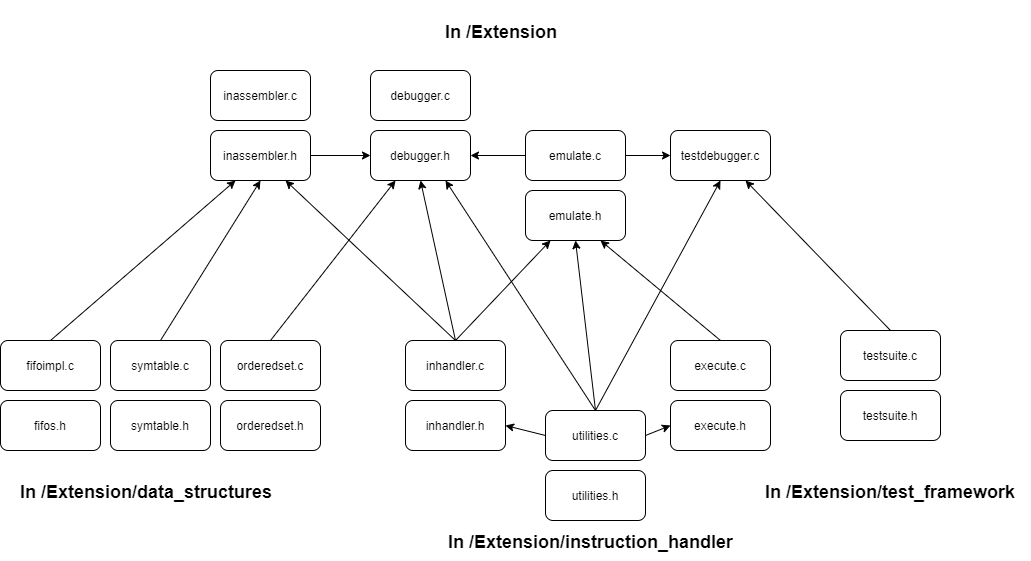
\includegraphics[width=17cm]{IncludesDiagramDebugger.png}
    \caption{Debugger Dependencies Diagram}
\end{figure}

Support for block data transfer instructions is an extension of both the emulator and assembler that allows for processing this fifth kind of instruction. This means our emulator and assembler now support instructions with mnemonics (LDM, STM) fully, in the same way that the other four instructions described in parts 1 and 2 are supported. The dependencies diagram for block data transfer is the same as the assembler.


\section{Extension Implementation And Challenges}
The debugger was implemented in the file debugger.c. User input is read utilizing fgets, and then tokenized by strtok, and then finally categorized by enum type command, utilizing a lexer function lexercommand. The main function opens the binary and assembly file, loads the binary file onto the memory layout, and puts the assembly instructions in a char * array, so it can be easily printed. Then it runs the debug function. The debug function is the main debugging function which runs the debugger loop, which first reads the debugger command, and then depending on the enum type, delegates the work to the command functions. \\

The command functions RUN (r) and NEXT (n) use the emulator function emulateInstruction, which runs the emulator exactly for one instruction. This would mean that we would have to take into account the pipeline with the debugger, because when we want to, for example, use the command NEXT (n), we want it to execute that line, not put it in the pipeline and wait until its full. Thus, the debugger command functions fill up the pipeline and then executes the current line.\\

Breakpoints and watchpoints are implemented utilizing an ordered set, since we can't have duplicates, and only need to add, remove, and check if it contains a specific breakpoint. RUN and NEXT take into account these structures whenever they are executed. \\

Commands PRINT, HELP, and QUIT, are pretty self-explanatory: print just checks the register array and data array and prints accordingly, HELP uses printf to print a list of commands, and QUIT prompts the user to press [y/n] to see if they really want to quit, and if yes, breaks the debugger loop.\\

The biggest challenge we encountered while making the debugger was handling the many edge cases that user input entails, and how to handle them. Also, thinking of how to approach the problem of implementing a parser without prior knowledge was a hard task, and we approached it by making the commands as simple as possible, and putting the HELP command to guide users to see what each letter command does. \\

The Block Data Transfer instruction implementation is modification of already existing files of the assembler and emulator. The file inassembler.c was populated with extra functions which work with instruction mnemonics and various suffixes which are used only for Block Data Transfer type. Some functions were modified, such as getCondSuffix, which now has extra case, when instruction mnemonic can be up to seven characters long. Also a syntactical sugar was added. Special register names, such as "sp", "lr" and "pc" are now supported. One of the challenges is that the syntax of the instruction contains the register list, which can be specified as a comma separated list or dash separated range or both, For example "\{r0,r1,r2\}" or "\{r0-r2\}" or "\{r0-r1,r2\}" are equivalent and all cases must be supported. The function assembleBlockDataTransfer, just like any other "assemble" instruction collects the components of the 32-bit number, such as flags, register numbers, register list and condition code and then creates the resulting 32-bit value with the aid of logical shifting and the usage of bit-wise "or" operation. \\

The next part is emulator expansion. Implementation started with adding some auxiliary functions in the file inhandler.c, such as boolean flag getters, the base register getter and the function getRegisterList, which returns heap-allocated array of indices of the registers which are present in the register list part of the instruction. This auxiliary functions were used in the function executeBlockDataTransferInstruciton, which performs the multiple transfer operation. One of the challenges here was to insure that the lowest registers are always transferred into the lowest addresses in the memory. As a result, the counter intuitive approach was used, where the values are not pushed like in a real stack but inserted inside the earlier computed location.  \\

One of the limitations of the achieved implementation is that it cannot fully support the usage of the caret character at the end of the register list syntax. This character if present, sets the S flag, which works with privileged modes of the ARM. Since the proposed implementation assumes that the emulated ARM processors works in the user mode, this character acts as a condition to ignore this instruction. Meanwhile in the real ARM it will be executed in certain modes. However, this character is supported and parsed by the assembler, though it is not useful under the limitations described above. \\

\section{Extension Testing}

The debugger was first tested informally by handling user inputs and testing edge cases through just running the program with any of the test cases provided in the test suite. Then, in order to formalize our testing, we decided to put our user inputs in an input files, which can be found on the testfiles directory. This way, we can test really long-ended debugger utilization examples. Testdebugger.c contains various test functions that tests specific command functions, and a last really long user input, testing factorial.s, and utilizing all commands. We believe that to a certain extent, this testing was indeed effective as it allowed us to see exactly what command was working incorrectly. However, the debugger  has too many user input edge cases that it is really hard to test all of them, and due to this, testdebugger.c is quite limiting.\\

Block Data transfer instruction support was tested by assembling and emulating several programs and then examining the non-zero memory and registers values output. It was a high level testing of the whole application in general. Programs initialised the data or registers and then executed instruction which transferred multiple register values to memory (STM) and vice versa (LDM). Although the tests might not be fully exhaustive, The output matched expectations and the program showed correct behaviour. \\

\section{Group Reflection On The Task}

At the start, with the emulator, our group did not coordinate well and did not have a goal in mind, largely due to the inability to brainstorm a way to start the emulator, and poor coordination. After the emulator, we decided to ponder and split the tasks of the assembler the best way possible, and through coordination and communication we were able to do the assembler quite efficiently. For the extension we decided to keep the same mentality and split the tasks in two groups and then merge later, leading again to an effective result. \\

Things we would keep the same would be having a preparatory meeting before starting to work to brainstorm how to split the tasks and making sure everyone is up to date with the specification. This helped us tremendously in our workflow and made sure everyone was actively contributing to the project. Something that was missing in our project was active communication after every change in the code. This led to miscommunication in our part and having to remove duplicate code.
\section{Individual Reflections}
\subsection{Diego (dc1020)}
I enjoyed working with my group, and I didn't encounter any major problems with any of them. They were all friendly and willing to discuss anything related to the project. I would say that for this particular project, I was too eager to write code, which helped on getting the project finished on time, however, it did lead to adequate communication on my end, as I would not comment on all programming changes. Regardless, I did learn a really good amount on what I need to do when working in a group, and also how to document and make our code more maintainable and readable.
\subsection{Norberto (nm920)}
I feel I learnt a lot with this project, not only did it help me learn and gain a deep understanding in C programming, which at first I was worried I was going to have trouble keeping up with my teammates, but it also taught me how to work in a group and how to coordinate with other people. With the help of Diego and Andrey, who are computing students, I was able to understand the ARM assembly language much quicker given they had already done the computer architecture course. I felt this was very useful in getting us going in the beginning as Agustin and I were just only starting the architecture course. Overall I really enjoyed working with everyone and I think we worked well together. 

\subsection{Andrey (ap4220)}
Overall, I enjoyed working with Diego, Norberto and Agustin. My teammates are friendly and hardworking. My weaknesses are that I am shy in communication and prefer to work independently. That led to some work being duplicated, so next time I will try my best to achieve better communication with the team. I learned a lot during this project, not only in programming skills or using the tools, but also how to work together and achieve results on time.

\subsection{Agustin (as1920)}
At the start of the project, without having any knowledge of Assembly, I was worried that I might not be able to help my team as much as Diego and Andrey (who are Computing students). So, at first, I helped with tasks that didn't require Assembly knowledge. One other weakness is that I tended to work with those who I knew already, so for the next project I will be more open to work with everyone. I believe my main strength was that I tried to help as much as possible, and that I always tried to work collaboratively. Overall, I really enjoyed working with Diego, Andrey and Norberto, since they were all hardworking and approachable.

\end{document}
